\documentclass[10pt]{beamer}
\mode<beamer>{%
  \usetheme[]{CambridgeUS}}
\usepackage{geometry}
\usepackage{tikz}
\def\checkmark{\tikz\fill[scale=0.4](0,.35) -- (.25,0) -- (1,.7) -- (.25,.15) -- cycle;} 
\usepackage{fancybox}
\usepackage{setspace}
\author{Devin Judge-Lord}
\begin{document}


\begin{frame}
\frametitle{Theory}
Do campaigns calling attention to agency actions influence \\(1) the policymaking environment or \\(2) policy outcomes? 

\bigskip

\small
\begin{tabular}{c c l c c}
\centering
& &  \fbox{Public attention campaign} & \\
& &  $\downarrow \downarrow \downarrow \downarrow \downarrow \downarrow \downarrow \downarrow \downarrow \downarrow \downarrow \downarrow \downarrow \downarrow \downarrow \downarrow \downarrow \downarrow \downarrow \downarrow \downarrow$ &  \\
\fbox{Lobbying} & $\Rightarrow$ & \textit{Policymaking  environment} & $\Rightarrow$ & \fbox{Policy change}\\
 & & - Perceived: \\
 & & - - H1 Threat of sanction\\
 & & - - H2 Threat of reversal\\
 & & - - H3 Right thing to do \\
 & & - - - 3.1 Public accountability \\
 & & - - - 3.2 Political accountability \\
 & & - - - 3.3 Statutory mission \\

\end{tabular}

\end{frame}


\begin{frame}
\frametitle{Design}
Do mass-comment campaigns influence \\(1) the policymaking environment or \\(2) policy outcomes? 
\bigskip

\small
\begin{tabular}{l c l c l}
\centering
& &  \fbox{Mass comment(s)} & \\
& & =\{$Ask1, \ Ask2$\}\\
& &  $\downarrow  n = \{1, >1000\}  $ &  \\
\fbox{Main comment} & $\Rightarrow$ & \textit{Policymaking  environment} & $\Rightarrow$ & \fbox{Policy change}\\
=\{$Ask1 + Ask2$\} & & Reported: & & - Granted \{$Ask1, Ask2$\}\\
& & - H1 Threat of sanction & & - Discussed \{$Ask1, Ask2$\} \\
& & - H2 Threat of reversal \\ 
& & - H1-3 Effect of comments\\
& & - H1-3 Effect of media\\
& & - H1-3 Effect of principals\\
& & Observed:\\
& & - H1-2 Letters from Congress\\
& & - H1-2 White House Attention\\
\end{tabular}

\end{frame}







\begin{frame}

\tiny

1. \textbf{Who is likely to participate in this notice-and-comment process?}

1.1 Do you have formal coalition partners? If so, please list them:

\fbox{\color{gray} ..............................................}


1.2 Who else is likely to comment \textit{in alignment} with your goals:

\fbox{\color{gray} ..............................................}

1.3 Who is likely to comment \textit{in opposition} to your goals:

\fbox{\color{gray} ..............................................}

Other likely commenters (neither aligned nor opposing): 

\fbox{\color{gray} ..............................................}

About how many total comments do you estimate will be received:

\fbox{\color{gray} ..............................................}

If your coalition is mobilizing citizen comments, how many do you anticipate mobilizing: 

\fbox{\color{gray} ..............................................}

\bigskip


2. \textbf{Why are you participating in this notice and comment process?}


In general: 

\fbox{\color{gray} ..............................................}

2.1 Briefly describe any procedural aims or complaints:

 \fbox{\color{gray} ..............................................}

2.2 Briefly describe any substantive goals:

\fbox{\color{gray} ..............................................}

\begin{tabular}{l c c c}
& Probability & Desired & Undesired \\
\hline\\
Withdrawal & \fbox{\color{gray} XX}\% & \fbox{\checkmark} & \fbox{\checkmark}  \\
Delay & \fbox{\color{gray} XX}\% & \fbox{\checkmark}& \fbox{\checkmark}  \\
Major revision & \fbox{\color{gray} XX}\% & \fbox{\checkmark} & \fbox{\checkmark} \\
\fbox{\color{gray} Other}  & \fbox{\color{gray} XX}\% & \fbox{\checkmark}  & \fbox{\checkmark}  \\
\ovalbox{\color{blue} Add potential outcome}\\
\end{tabular}

\end{frame}
\begin{frame}
\tiny
2.3 Please describe any specific potential revisions, including specific hopes, fears, and expectations, ideally specific bits of draft text that may change. Please check changes targeted by your coalition. For example any of the hoped policy changes that you suggest and any feared policy changes you argue against.

\bigskip

\begin{tabular}{c c c c c | c}
Did you lobby & Current & Potential & \multicolumn{2}{c}{\underline{Probability of change (your guess)}} & Was this on this issue?\\
for this change?& text& text & Without comments & With comments & [AFTER FINAL PUBLISHED]\\
\hline\\
\textbf{Hopes:} &\\
(1) \fbox{\checkmark}  & \fbox{\color{gray} Old text} & \fbox{\color{gray} New text} & \fbox{\color{gray} XX}\% & \fbox{\color{gray} XX}\% & Yes \fbox{\checkmark} No \fbox{\checkmark} Partial \fbox{\checkmark}\\
 \\
\ovalbox{\color{blue} Add hope}\\
\hline\\
\textbf{Fears:} &\\
(1) \fbox{\checkmark}  & \fbox{\color{gray} Old text} & \fbox{\color{gray} New text} & \fbox{\color{gray} XX}\% & \fbox{\color{gray} XX}\% & Yes \fbox{\checkmark} No \fbox{\checkmark} Partial \fbox{\checkmark}\\
 \\ \ovalbox{\color{blue} Add fear}\\
\hline\\
\textbf{Other expectations:} &\\
(1) \fbox{\checkmark}  & \fbox{\color{gray} Old text} & \fbox{\color{gray} New text} & \fbox{\color{gray} XX}\% & \fbox{\color{gray} XX}\% & Yes \fbox{\checkmark} No \fbox{\checkmark} Partial \fbox{\checkmark}\\
 \\
\ovalbox{\color{blue} Add expectation}\\
\end{tabular}

\end{frame}






\end{document}


\section{Outcome Measures}

\subsection{Goals Achieved}

The primary outcome is whether the organization achieved its goals. As priors and goals are stated for both the treatment and control rules in the survey that each organization will be asked to fill out, I can assess the difference between treated and untreated rules and whether the number of comments (dosage) is associated with the number of goals achieved. 

\subsection{Attention and issue framing}
I will use text analysis to measure three outcomes: First, did the agency respond to the concerns raised in the comments? Comparability requires that the mobilizing organization either submit their own comment (which often more technical than mobilized comments) on both treatment and control rules or submit on neither. As agencies are only required to respond to comments that they deem ``substantive,''  If the mobilizing organization submitted their own comment, response to mobilized comments may be measured as the difference in the length of response in treated and untreated rules. 

Second, comparing the preamble of the final rule to that of the draft, did the agency use more of the words and phrases matching those in the comments? Rule preambles are non-binding texts that frame the aims of the rule and the response to comments.  If the preambles of treated rules are more likely to include words or phrases from the organizations messaging and mobilized comments, this may indicate agency attention to their demands.\footnote{Recall that  treated and untreated rules both receive at least one comment with the organization's messaging but only treated rules receive a high dosage of it.}

Third, did the agency adopt language from comments into the text of the policy itself? It is unlikely that language from citizen comments will be sufficiently technical to be adopted into a rule. However, a higher dosage of public comments may make the more technical and legalistic comments of associated organizations more influential.

Each of these could be dummy variables or continuous measures based on the number of words in the agency response and number of new words and length of new phrases adopted from the comments into the preamble or rule. 

For example, figure \ref{ejlogitagencies} presents results from a logit model, showing the probability that a final rule will include the phrase ``environmental justice'' when the proposed rule did not but comments did. Many agencies rarely address environmental justice issues, but for those that do, the phrase being raised in comments is correlated with it being added to the rule. However, there are many reasons why this may occur. If whether environmental justice concerns were raised in comments or not could be experimentally manipulated, this could offer evidence about the causal effect.

\begin{figure}[ht!]
\caption{Proposed Rules Not Addressing Environmental Justice}
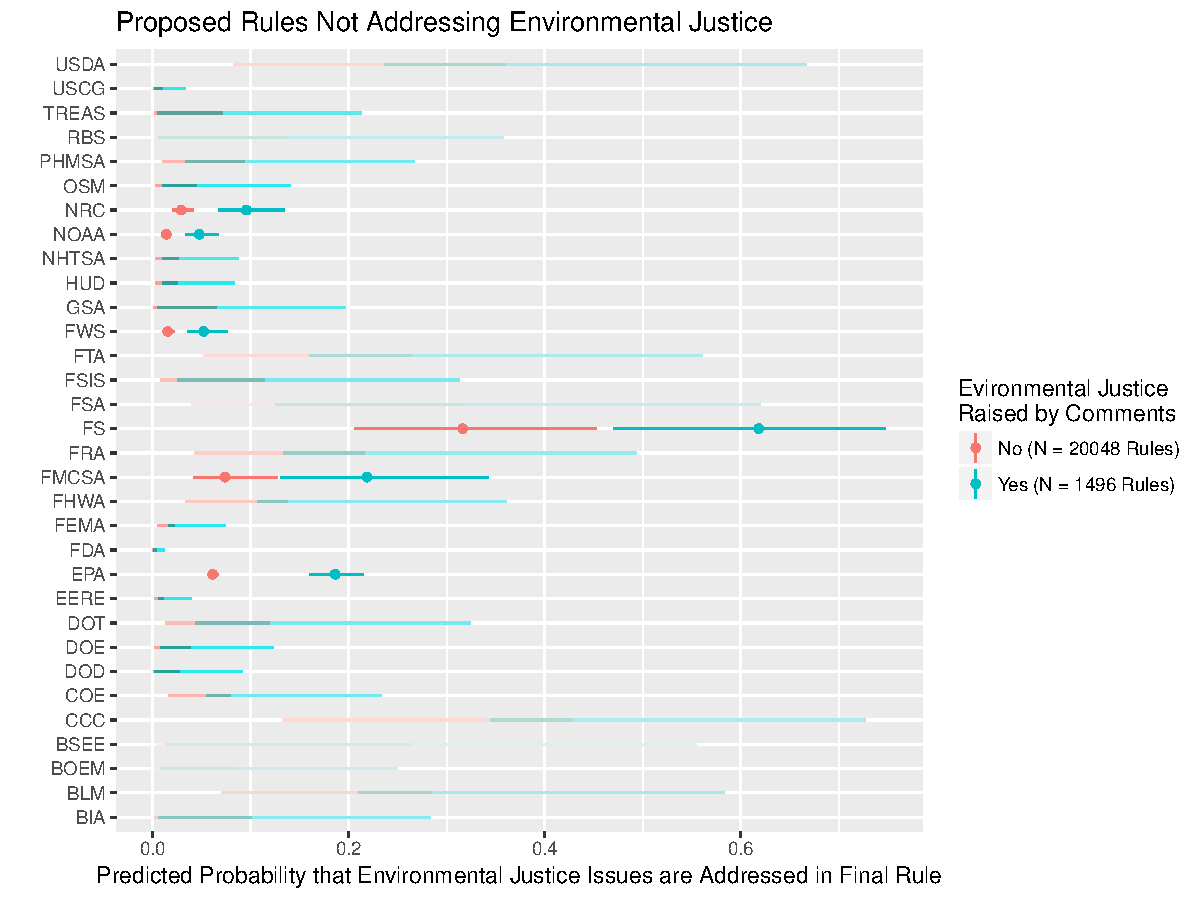
\includegraphics[width = \textwidth]{ej_prprob_by_agency.pdf}
\label{ejlogitagencies}
\end{figure}







\section{Identifying Mechanisms}

It may be impossible to identify the causal mechanisms that lead rule-writers to change policy.
I aim to assess comments' potential direct and indirect influence through agency records of internal and external communication about the rulemaking process and through interviews of rule-writers themselves. 

% \subsubsection{Why, agencies respond (science, fairness, representation, threat | agency identity)}
% Given prior expectations, assess treatment effects on agency decisions.

\subsection{Direct: Bureaucrat perceptions}

Rules are often on such technical questions that it is difficult to know where public opinion lies. One possible mechanism by which comments may influence rule-writers is by subtly reshaping their perceptions of the public will and the appropriate course of action for a public servant. I aim to identify ways in which mass public comment campaigns shape the thinking of and conversation among rule-writers in two ways. First, I will obtain records of internal correspondence about the rulemaking process in general and the response to comments in particular through a Freedom of Information Act (FOIA) request. Second, I will attempt to interview rule-writers. I will ask general questions about the particular rulemaking process and the reasoning behind any changes. If subjects mention public comments, I will ask what was compelling about the comments? This may not be an objective measure of these mechanisms, but it may be the closest one can get to knowing how public comments directly affect rule-writers' perceptions. 

\subsection{Indirect: External attention}

Public comment campaigns may also be effective through indirect causal pathways. Instead of comments directly mobilizing bureaucrats' beliefs about public opinion and the appropriate course of action for a public servant, they may attract the attention of political principals. The most relevant political principals are members of Congress and the President. Communications from members of Congress or the White House may affect beliefs about public opinion and the appropriate course of action for a public servant. Such communication may also signal potential consequences, such as changes to a program's budget, of the different courses of action.

I will measure congressional attention by (1) mentions of the rule in congressional testimony within 1 year of the proposed or final rule (this is rare), (2) filing FOIA requests for any communication between members of Congress and agency staff about the proposed rule (slightly more common), and (3) the importance rule-writers place on congressional attention when interviewed. I will measure attention from the White House by (1) whether the White House Office of Management and budget requires substantial changes to the rule,  (2) by filing FOIA requests for communication between the white house and agency staff regarding the rulemaking process, and (3) the importance rule-writers place on attention from the White House when interviewed. 

External attention has two forms: general attention, which may increase with increased salience caused by a mass-commenting campaign, and specific attention referencing public comments as a reason for the attention.  

